\documentclass[mathserif,serif]{beamer}

\usepackage{graphicx}
\shorthandoff{=}

%\setbeamertemplate{blocks}[rounded][shadow=true]
\setbeamertemplate{background canvas}[vertical shading][bottom=white,top=structure.fg!25]

\mode<presentation>

\newcommand {\framedgraphic}[2] {
    \begin{frame}{#1}
        \begin{center}
            \includegraphics[width=\textwidth,height=0.8\textheight,keepaspectratio]{#2}
        \end{center}
    \end{frame}
}


\title{SWOP iteratie 1}
\author{Pablo en Co (groep 2)}
\institute{KU Leuven}
\date{2015}

\begin{document}

  \frame{\titlepage}

  \begin{frame}{High Level}
      \begin{columns}[c]
        \begin{column}{0.33\textwidth}
          \begin{center}
            GRASP:\\
            Controller
          \end{center}
        \end{column}
        \begin{column}{0.33\textwidth}
            \includegraphics[width=\textwidth,height=0.6\textheight,keepaspectratio]{../../diagrams/high_level_uml.eps}
        \end{column}
        \begin{column}{0.33\textwidth}
          \begin{center}
            Patterns:\\
            Facade
          \end{center}
        \end{column}
      \end{columns}
          \begin{center}
            \begin{itemize}
              \item Session controller = functionaliteit per use-case
              \item Facade controller = aanspreekpunt voor domain
              \item UI werkt niet rechtstreeks met domain
            \end{itemize}
          \end{center}
  \end{frame}

  \begin{frame}{Facadecontroller}
      \begin{columns}[c]
        \begin{column}{0.80\textwidth}
      \includegraphics[width=\textwidth,height=0.5\textheight,keepaspectratio]{../../diagrams/facade_uml.eps}
        \end{column}
        \begin{column}{0.20\textwidth}
          \begin{center}
            Patterns:\\
            Facade\\
            \vspace{1cm}
            GRASP:\\
            High Cohesion\\
            Indirection
          \end{center}
        \end{column}
      \end{columns}
      \begin{center}
        \begin{itemize}
        \item Duidelijke verantwoordelijkheid:
        \item Wrapping en unwrapping
        \item Bescherming van domain
        \item Zit tussen domain en UI
        \end{itemize}
      \end{center}
  \end{frame}

  \begin{frame}{Task interpretatie}
      \begin{center}
      
\includegraphics[width=\textwidth,height=0.5\textheight,keepaspectratio]{../../diagrams/task_dfs.eps}
        \begin{itemize}
        \item Task beslist welke status te gebruiken
        \item Status beslist over functionaliteit van Task
        \item Status wordt berekend bij opvraging
        \end{itemize}
      \end{center}
  \end{frame}

  \begin{frame}{Project}
      \begin{center}
      \includegraphics[width=\textwidth,height=0.5\textheight,keepaspectratio]{../../diagrams/project_dfs.eps}
        \begin{itemize}
        \item Status hangt enkel af van taken ...
        \item ... en geen specifieke functionaliteit per status
        \item $\Rightarrow$ Geen extra klassen nodig
        \item $\Rightarrow$ Enkel 'isX' checks
        \end{itemize}
      \end{center}
  \end{frame}

  \begin{frame}{Domain}
      \begin{columns}[c]
        \begin{column}{0.70\textwidth}
      \includegraphics[width=\textwidth,height=0.6\textheight,keepaspectratio]{../../diagrams/domain_uml.eps}
        \end{column}
        \begin{column}{0.30\textwidth}
          \begin{center}
            GRASP:\\
            Creator\\
            High Cohesion\\
            Information-Expert\\
            Low Coupling\\
          \end{center}
        \end{column}
      \end{columns}
      \begin{center}
        \begin{itemize}
        \item Task $\leftarrow$$\rightarrow$ Status
        \item ... geen bi-directional relatie nodig voor 'dependsOn'
        \item Task geen kennis nodig van project
        \end{itemize}
      \end{center}
  \end{frame}

  \begin{frame}{Create Task}
      \begin{center}
      \includegraphics[width=\textwidth,height=0.6\textheight,keepaspectratio]{../../diagrams/sequence_createTask_uml.eps}
        \begin{itemize}
        \item ProjectWrapper
        \item ProjectData
        \item createTaskFor(projectWrapper, projectData)
        \end{itemize}
      \end{center}
  \end{frame}

  \begin{frame}{Testing}
      \begin{center}
      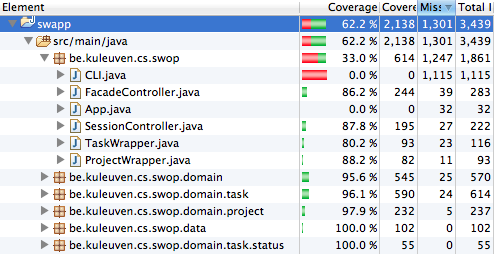
\includegraphics[width=\textwidth,height=0.6\textheight,keepaspectratio]{code_coverage.png}
        \begin{itemize}
        \item Unit tests per klasse
        \item Use case tests $\rightarrow$ Testing UI
        \item Scenario test
        \item Fuzz testing $\rightarrow$ Button masher UI
        \end{itemize}
      \end{center}
  \end{frame}

% etc
\end{document}




%%% Local Variables:
%%% mode: latex
%%% TeX-master: " RET"
%%% End:
